\documentclass[hidelinks]{article}
\usepackage[utf8]{inputenc}
\usepackage{filecontents, hyperref}
\usepackage{graphicx,hyperref}
%\usepackage[round]{natbib}
\usepackage[style=authoryear, backend=biber
			, natbib = true]{biblatex}
%\addbibresource{paper.bib}
\bibliography{paper.bib}
\usepackage{dcolumn}
\usepackage{booktabs}
\usepackage{setspace}
\usepackage{color,soul}
\usepackage{comment}
\usepackage{amsfonts}
\usepackage{geometry}
\usepackage{caption}
\usepackage{titlesec}
\usepackage{sectsty}

\setlength{\parskip}{1.2ex}
\setlength{\parindent}{2em}
\usepackage{url}

%\let\origfootnote\endnote
%\renewcommand{\endnote}[1]{%
%   \renewcommand\footnotesize\normalsize%
%   \origfootnote{#1}}

% Sans-Serif font for sections
\allsectionsfont{\sffamily}
% Change spacing of \paragraph command
\makeatletter
\renewcommand{\paragraph}{%
  \@startsection{paragraph}{4}%
  {\z@}{0.25ex \@plus 0.5ex \@minus .2ex}{-1em}%
  {\normalfont\normalsize\bfseries}%
}
\makeatother


\begin{document}

\title{Using Machine-coded Event Data for the Micro-level Study of Political Violence}
\author{Jesse Hammond (Corresponding Author) \\
\let\thefootnote\relax\footnote{Jesse Hammond is a doctoral candidate in Political Science at the University of California at Davis, 1 Shields Avenue, Davis CA 95616, and the University of Konstanz (jrhammond@ucdavis.edu +01 209 479 0625). Nils B.~Weidmann is Professor of Political Science at the University of Konstanz, Box 216, 78457 Konstanz, Germany (nils.weidmann@uni-konstanz.de +49 7531 88 5676)}
Nils B.~Weidmann}
\date{\today\\[5mm]Word count: 3,994 not including figures or abstract\\[5mm]
Keywords: Event data, political violence, micro-level analysis, GDELT, GIS}

\maketitle


\begin{abstract}\textsl{}
Machine-coded datasets likely represent the future of event data analysis. We assess the use of one of these datasets--GDELT--for the micro-level study of political violence by comparing it to two hand-coded conflict event datasets. Our findings indicate that GDELT should be used with caution for geo-spatial analyses at the subnational level: its overall correlation with hand-coded data is mediocre, and at the local level major issues of geographic bias exist in how events are reported. Overall, our findings suggest that due to these issues, researchers studying local conflict processes may want to wait for a more reliable geocoding method before relying too heavily on this set of machine-coded data.
\end{abstract}

\doublespacing 

The introduction last year of the Global Database of Events, Language and Tone (GDELT, \citealt{leetaru13gdelt}) has caused a stir in academic and policy communities alike. With a quarter of a billion observations, a 35-year temporal span, and daily updates through automated coding, the advantages are manifold. Using automatic geo-referencing routines, event data not only come with temporal coordinates, but are also tagged with geographic coordinates. As compared to the previous generation of machine-coded event datasets, this makes the new generation of event data suitable for the micro-level, geo-spatial analysis of political events. In this paper, we assess the use of these datasets for micro-level studies, focusing in particular on political violence where spatial analysis has become a widely-used approach. While there has been earlier work attesting to the validity of machine-coded events, our focus in this paper is the quality of geo-localization. In other words, we ask whether machine-coded event datasets can approximate the spatial pattern of a conflict to a reasonable extent.  

To answer this question, we correlate the spatial patterns of violence as coded by two established human-coded event datasets to those given by GDELT. Since these datasets attempt to code the same type of event, and use many of the same sources to code event data, we expect the correlation to be high. Yet, this is not what we find: our spatial-temporal analysis shows that GDELT does correlate significantly with the other event datasets, although these correlations remain fairly low. However, when we collapse our data to a time series---eliminating the geographic dimension---correlations become much stronger. This suggests that spatial disaggregation accounts for much of the disagreement between machine- and human-coded data. To further explore this, we analyze how spatial remoteness accounts for the mismatch between the data. The results confirm a geographic bias; whereas GDELT over-reports violence close to the capital, the opposite applies in remote locations. This is problematic, since we risk falsely associating civil war violence with urban areas \citep{kalyvas04urban}. Despite the proven reliability of machine-coding techniques, our findings indicate that significant work is required in optimizing the automated geo-localization of event data. In the next section, we briefly sketch the development of event data in political analysis, before turning to our analysis and results, which focus on political violence more narrowly.

\section*{Automatic and Non-automatic Approaches to Event Coding}

The recent surge of academic interest in political violence has spurred the development of event data. An event dataset is one that lists individual acts or interactions along with precise coordinates. Event data have a history in political science; earlier approaches originated mostly in international relations, focusing on actions between states. Examples date back a few decades, and include the World Event Interaction Survey (WEIS, \citealt{mcclelland71world}) and the Conflict and Peace Data Bank (COPDAB, \citealt{azar80conflict}). Later, \citet{schrodt94keds} developed machine-assisted approaches to generate the same kind of data from news sources, which have been used in the creation of large international datasets such as the Kansas Event Data System KEDS \citep{gerner94machine}. Validity checks indicate that machine-coded events can match human-coded data with a high degree of accuracy regarding the substance of events and the actors involved \citep{schrodt94validity, best13tabari}.

A recent generation of event datasets combines new data with a sharper substantive focus. Most importantly, location plays a major role. Event datasets such as the Armed Conflict Location and Event Dataset ACLED \citep{raleigh10acled}, the Geo-referenced Event Dataset GED released by the Uppsala Conflict Data Program \citep{sundberg13introducing}, or the Social Conflict in Africa Database SCAD \citep{salehyan12social} all list events with precise spatial coordinates, making it possible to study patterns of violence as well cross-link the events to other spatial data \citep{gleditsch12richardson}. This was done to allow both cross-national and sub-national analysis of political violence, as for example in \citet{raleigh09population} or \citet{weidmann10predicting}. All these datasets rely largely on human coding of news reports, and thus require significant effort and time\footnote{Some new data initiatives still in development, such as the Social, Political, and Economic Event Data Project (SPEED, \url{http://www.clinecenter.illinois.edu/data/speed/}) and the Event Data on Armed Conflict and Security Project (EDACS, \url{http://www.conflict-data.org/edacs/index.html}), attempt to utilize the speed of machine coding with direct human oversight. We eagerly look forward to learning more about the advantages of this hybrid approach as these projects mature.}.

Further developments in machine coding attempt to generate a similar type of data. For example, the recent GDELT project applies automated coding techniques to the generation of event data from English language media reports, with the key addition of automated geo-coding. This results in a data product that largely relies on the same sources as the human-coded datasets (local and international sources from newspapers and newswires, usually provided through repositories such as LexisNexis and Factiva), but whose creation is fully automated. The machine coding approach is to define lists of actors and events, as well as the words identifying them in natural language. News reports are fed into a parser that identifies events based on the actor and event keywords given in the dictionaries.\footnote{See \url{http://eventdata.parusanalytics.com/data.html} for a more detailed description.} GDELT relies on the CAMEO event classification scheme to code events \citep{gerner02cameo}. Similarly, a simple lookup of place names is used for each event to extract location information from media reports \citep{leetaru13gdelt}. 

There are several reasons why machine coded events could diverge from human-coded ones. First, there may be differences regarding the events that are detected: the automated coding process may fail to pick up events, or code others that the human coder chose not to include. This could be due to ambiguous or non-standard language patterns describing events, but could also be due to the fact that human-coded datasets require background information on civil wars when coding events: the GED, for example, requires events to be explicitly linked to an ongoing civil war in order to be included in the dataset. Machine coding routines do not have this background knowledge, and rely entirely on information and keywords supplied in a single article. This latter effect should lead machine coding algorithms to be much less selective when it comes to the events included. Second, even if events are included in both data collections, these coding approaches may differ when it comes to the nature of the event. For example, discrepancies could exist in the coding of the attacker or the target of violence. Last, even with identical source data and coding techniques, locational discrepancies could exist due to issues with the geo-referencing process. Automated geo-referencing is far from straightforward; oftentimes, reports mention different locations, and it is difficult to discern which locational information in a report actually describes the event's location. For example, due to frequent mentions of the capital in news reports, a ``capital bias'' could occur that places many events wrongly in the country's most prominent city. 

This information, however, is key for the rapidly evolving micro-level analysis of violence \citep{kalyvas12micro}, which oftentimes relies on geographic information. How well does GDELT track variation in violence at the local level? Earlier work has analyzed the validity of machine-coding more generally \citep{schrodt94validity}, and there have been a few attempts to conduct similar analyses of GDELT in particular. A paper by \citet{arva13improving} compares GDELT to another event dataset---the commercial product ICEWS\footnote{See \url{http://www.lockheedmartin.com/us/products/W-ICEWS/W-ICEWS_overview.html} for more information.}---that relies on machine coding. However, this comparison is done at the country level, and therefore not particularly insightful for micro-level researchers. Another GDELT validation by \citet{ward13comparing} also uses ICEWS for comparison, but focuses on temporal trajectories at a fixed location, which again cannot tell us much about correspondence across space. Therefore, our analysis is the first attempt to probe GDELT's usefulness for micro-level research. The next section presents our approach and the results.


\section*{Data}

Our analysis compares GDELT to two other established datasets on political violence, the ACLED \citep{raleigh10acled} and GED \citep{sundberg13introducing}\footnote{For an in-depth discussion of the differences and similarities between GED and ACLED, see \citep{eck12ged}.}. To ensure overlap between these datasets, we analyze violence Africa between 1997 and 2008. Within this range, we further subset the data into only country-years during which at least one civil conflict was ongoing, as coded by the UCDP-PRIO armed conflict dataset \citep{themner13armed}. The resulting coverage for all three datasets includes 25 countries and 136 conflict-years. Within this range, we aggregate the three datasets at the level of cell-months, using uniform grid cells of approximately 55 kilometers on each side from the PRIO-GRID dataset \citep{tollefsen12priogrid}. Our dataset consists of 5,897 unique cells, with a total of 547,812 monthly observations.

Our comparison focuses on the presence or absence of conflict events at the cell-month level between these three datasets. As they ostensibly cover the same type of event, we are interested in seeing how similar subnational GDELT coverage of civil war violence is to the more established hand-coded datasets. Since GDELT covers a much wider range of political events, we filter out those that fit the definition of civil war violence. Specifically, a GDELT event is kept if it meets the following criteria for information:
\begin{enumerate}
\item The event is classified as direct armed clash or battle;
\item The event location is geolocated at least at the administrative district or city level;
\item The initiator is identified generally as a government body, military organization, or insurgent group.
\end{enumerate}
This subsetting only requires event type, location, and actor, a bare minimum for event data analysis. For the hand-coded datasets, we also subset by event type (violent conflict event), and geographic precision (events coded at the city or district level). For a more in-depth explanation of our coding rules see Appendix A, and for the results of parallel analyses using alternative coding rules, see Appendix B. 

We also realize that these datasets, even when coding the same type of event, use different general rules in converting raw data to event records. The GED coding method attempts to create one record `per event', meaning that events lasting more than one day only count as one observation, and differs from the other two datasets in that it only codes events where at least one fatality is recorded, leading to a lower overall event count. The ACLED coding, on the other hand, codes what are essentially `event-days', with one observation per day that an event was ongoing. Finally, GDELT's automated coding system can vary as to how many observations correspond to one 'event', as it relies on specific pieces of information in a news article to determine whether two sources describe the same event. To control for this issue, we dichotomize monthly event-counts to a conflict variable (0/1), with 1 corresponding to cases where at least one event was reported in a given cell-month, and 0 otherwise. We also run our set of models on the raw event-count data, and find very similar results (Appendix C).

A final potential issue is that the three datasets use partly different sources. ACLED and GED do not have specific rules regarding what sources are used to code events: they rely primarily on newswire sources, but also use a wide variety of media and non-media sources to maximize coverage. GDELT, on the other hand, relies on a much more limited set of media sources, primarily four news streams available on LexisNexis: Agence France-Presse, Associated Press, BBC Monitoring Service, and Xinhua News Service (and Google News from 2002 onwards). In order to rule out the possibility that differences in the sources used account for potential discrepancies, we run a set of models on a subset of ACLED and GED that only includes events recorded by the four main media sources used by GDELT. We find virtually identical results (Appendix D).

\section*{Correlations Across Datasets}

Our first step is to compare time trends in event reporting, similar to the approach followed in other GDELT validation exercises. Figure \ref{fig:time series} displays aggregated time-series for GDELT, ACLED and GED for the period we examine, showing the total number of grid-cells experiencing one or more conflict events in a given month.

\begin{figure}[!htbp]
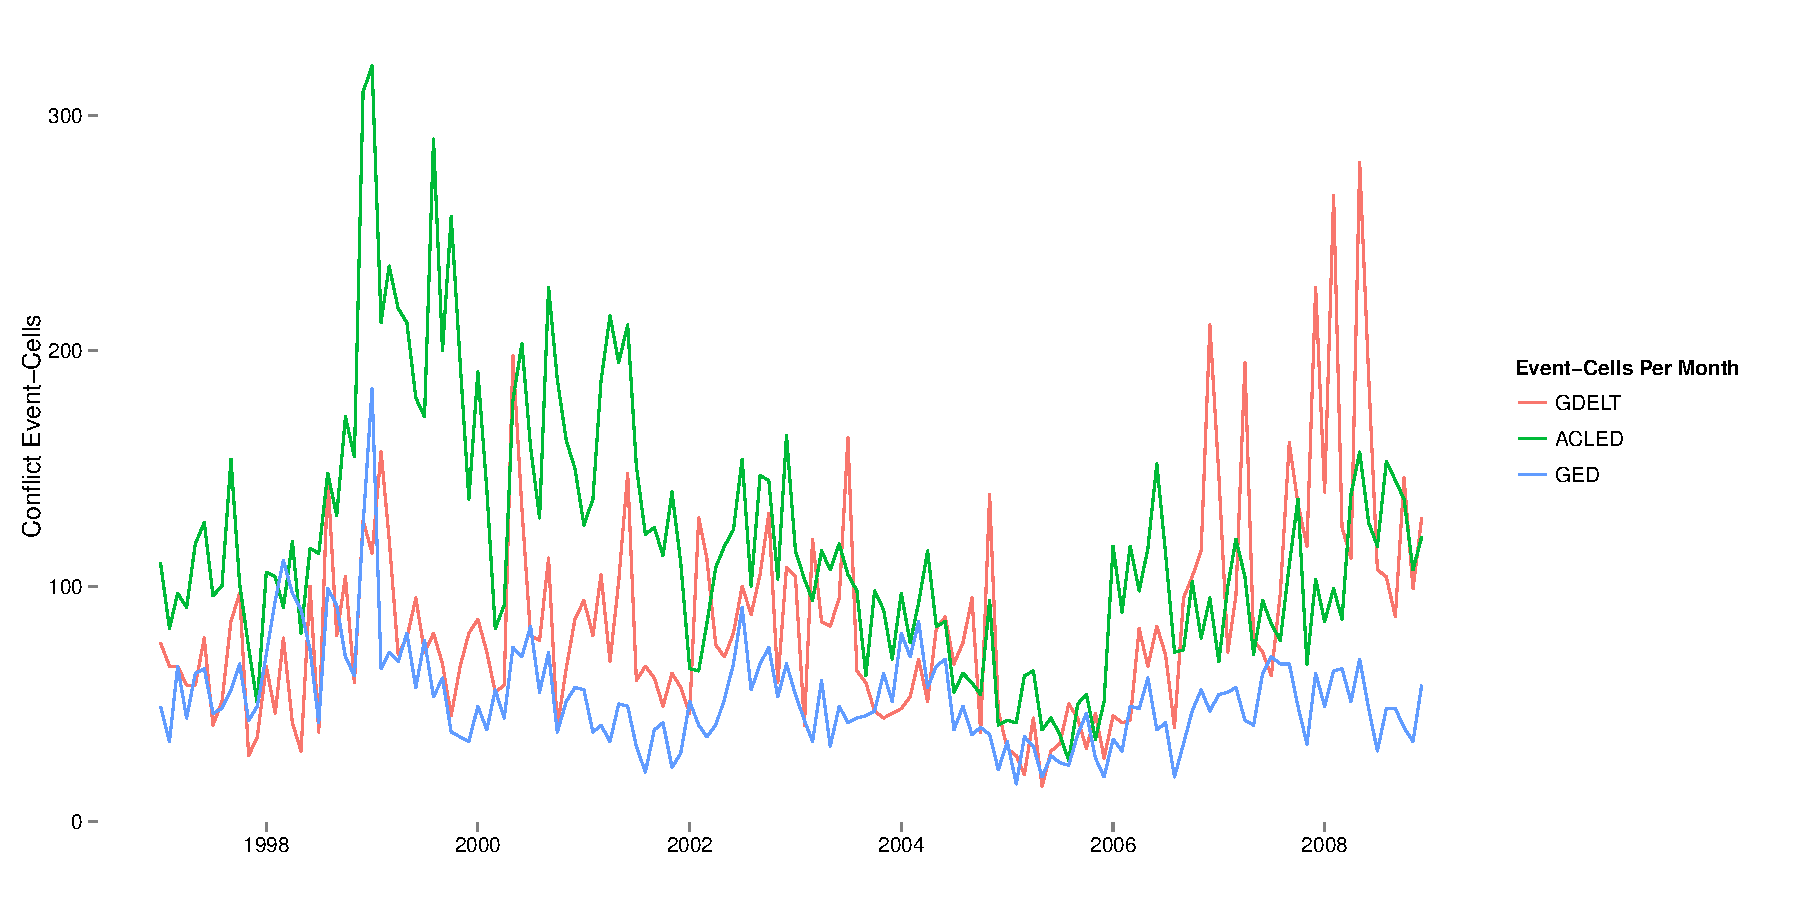
\includegraphics[width = 1 \textwidth]{EventTimeSeries.pdf}\\
\caption{Total events over time.}\label{fig:time series}
\end{figure}

When looking at the data as a time series (ignoring spatial variation), GDELT correlates with ACLED at 0.64, and with GED at 0.33. Overall, this is in line with previous findings that automated event coding can generally track hand-coded data \citep{best13tabari}, but the overall strength of the correlations remains modest. However, these correlations drop dramatically once we add the spatial dimension. At the grid-month level, GDELT correlates with ACLED at 0.26, and with GED at 0.20. A closer look at the confusion tables (Table \ref{tab:confusion}) reinforces this impression. While all datasets agree on the absence of conflict in the vast number of cases (top left cells), the majority of grid-cells that GDELT codes as experiencing conflict are not classified as such by either of the two datasets (bottom left cells), nor does GDELT pick up many of the cases that ACLED or the GED code as conflict (top right cells). Taken together, these figures provide evidence that the automated coding process GDELT uses to geolocate events may differ from human coders: even though it tends to code a similar set of events as ACLED and GED (as confirmed by the time trends above), it seems to have issues in placing those events in the same locations as human coders.

\begin{table}[!htbp] \centering 
\begin{tabular}{@{\extracolsep{5pt}}lcc|cc} 
& \multicolumn{1}{c}{ACLED = 0} & \multicolumn{1}{c}{ACLED = 1} & \multicolumn{1}{c}{GED = 0} & \multicolumn{1}{c}{GED = 1} \\ 
\hline \\[-1.8ex] 
GDELT = 0 & 538,541 & 5,552  & 540,494 & 3,589\\ 
GDELT = 1 & 2,398 & 1,331  & 2,906 & 823 \\ 
\hline \\[-1.8ex] 
N = 547,812 Cell-Months\\
\normalsize 
\end{tabular} 
 \caption{Confusion Matrices.}\label{tab:confusion}
\end{table} 

To further study how the correlations between the datasets vary over time and space, we visualize ``overlap'' between the datasets in Figures \ref{fig:correlations_time} and \ref{fig:correlations_space} below. The bars indicate the number of conflict cases identified by each dataset over time (Figure \ref{fig:correlations_time}) and space (Figure \ref{fig:correlations_space}). In each plot the overlapping area in the center represents the number of cases where both datasets code conflict (the true positives). Figure \ref{fig:correlations_time} pools all observations for a given month to create the plot. Figure \ref{fig:correlations_space} pools observations by cell, and orders the cells by distance from capital. Due to the large number of grid-cells (nearly 6,000), we subset the sample visualized in Figure \ref{fig:correlations_space} to only include grid-cells where both datasets report at least one conflict event in the same month.

\begin{figure}[!htbp]
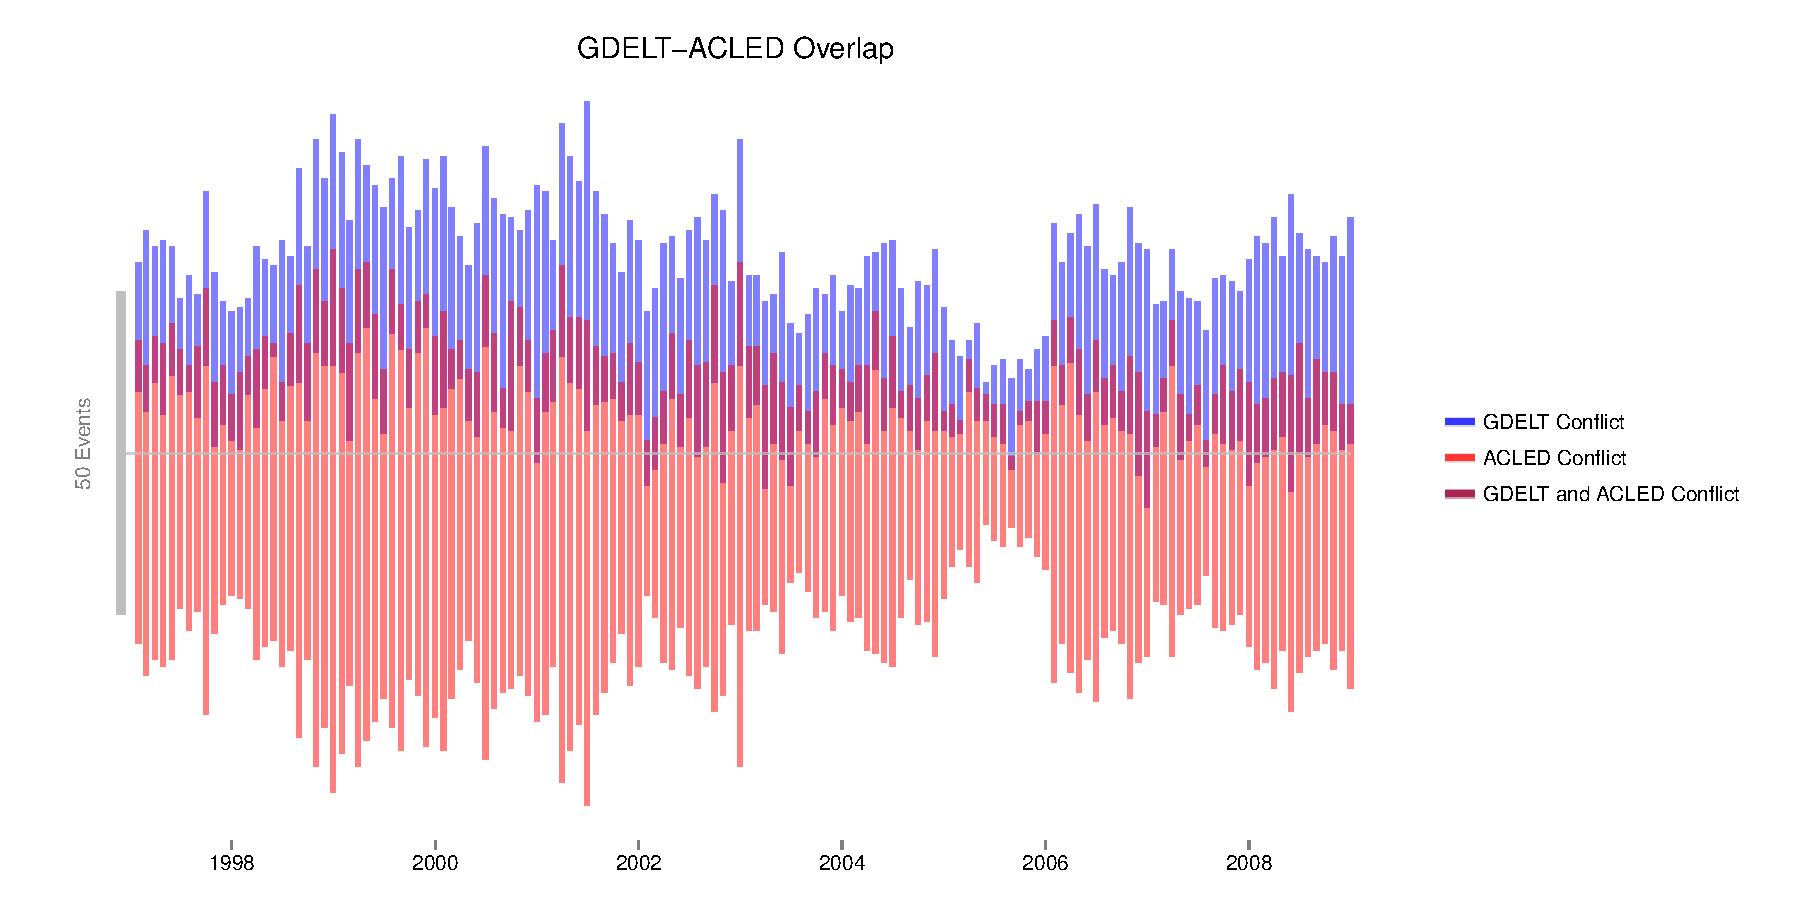
\includegraphics[width = 1 \textwidth]{timeACLED.pdf}\\
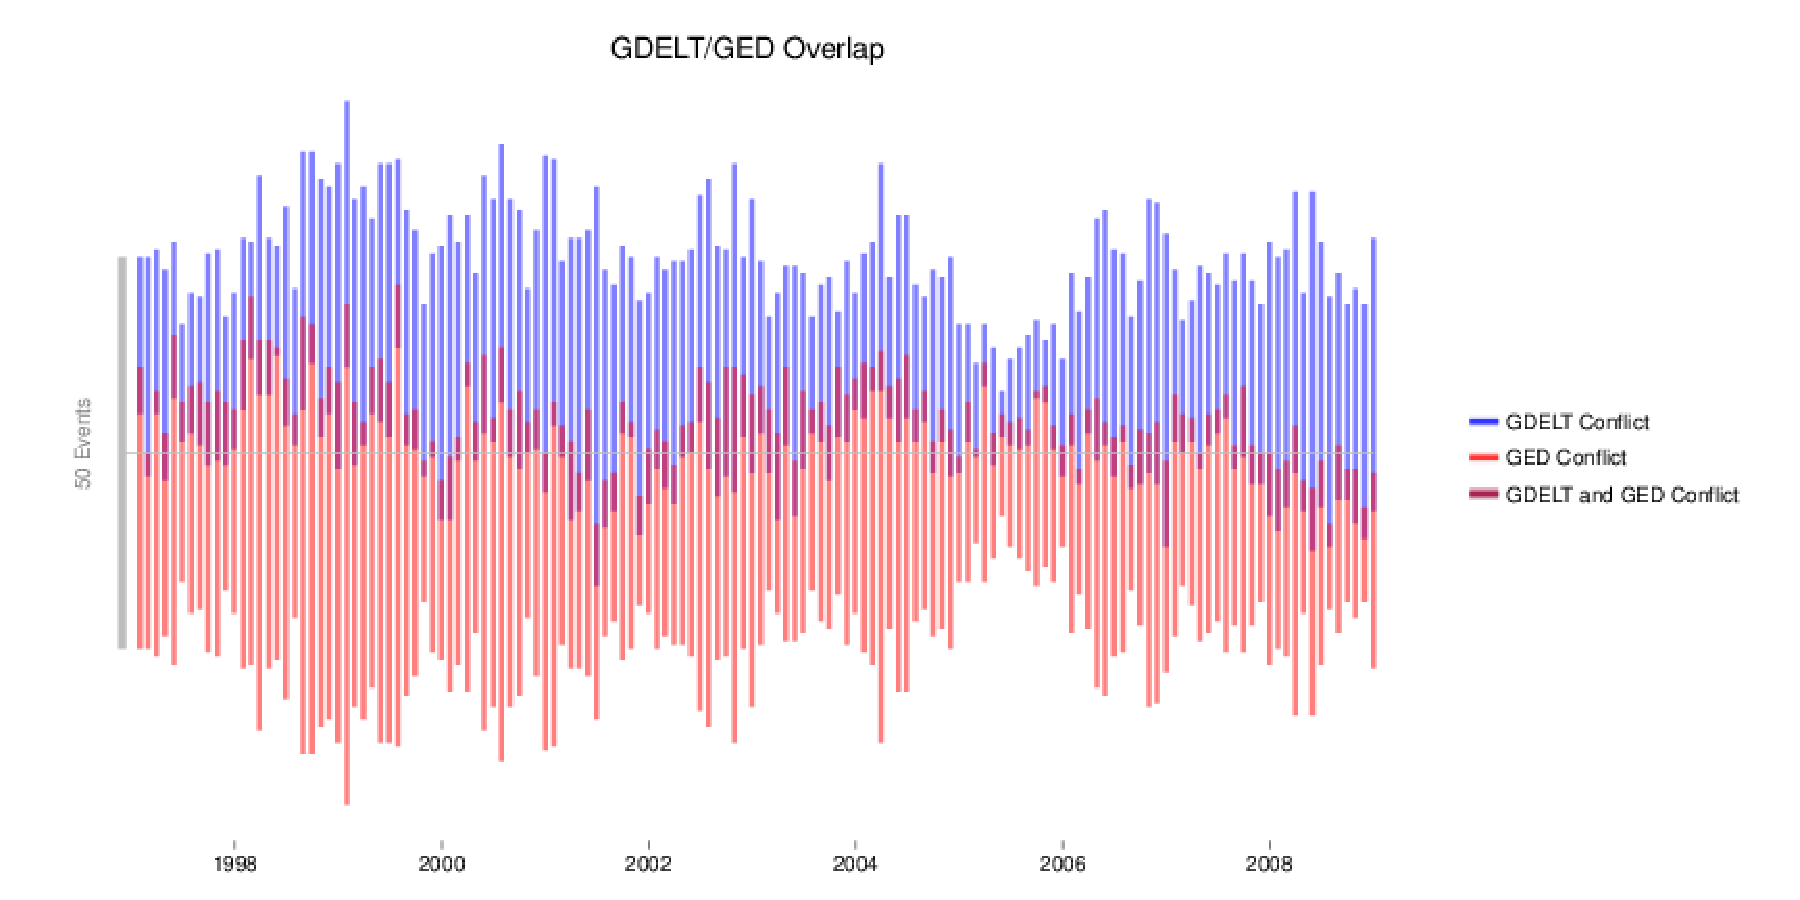
\includegraphics[width = 1 \textwidth]{timeGED.pdf}
\caption{Grid-cell events over time.}\label{fig:correlations_time}
\end{figure}

\begin{figure}[!htbp]
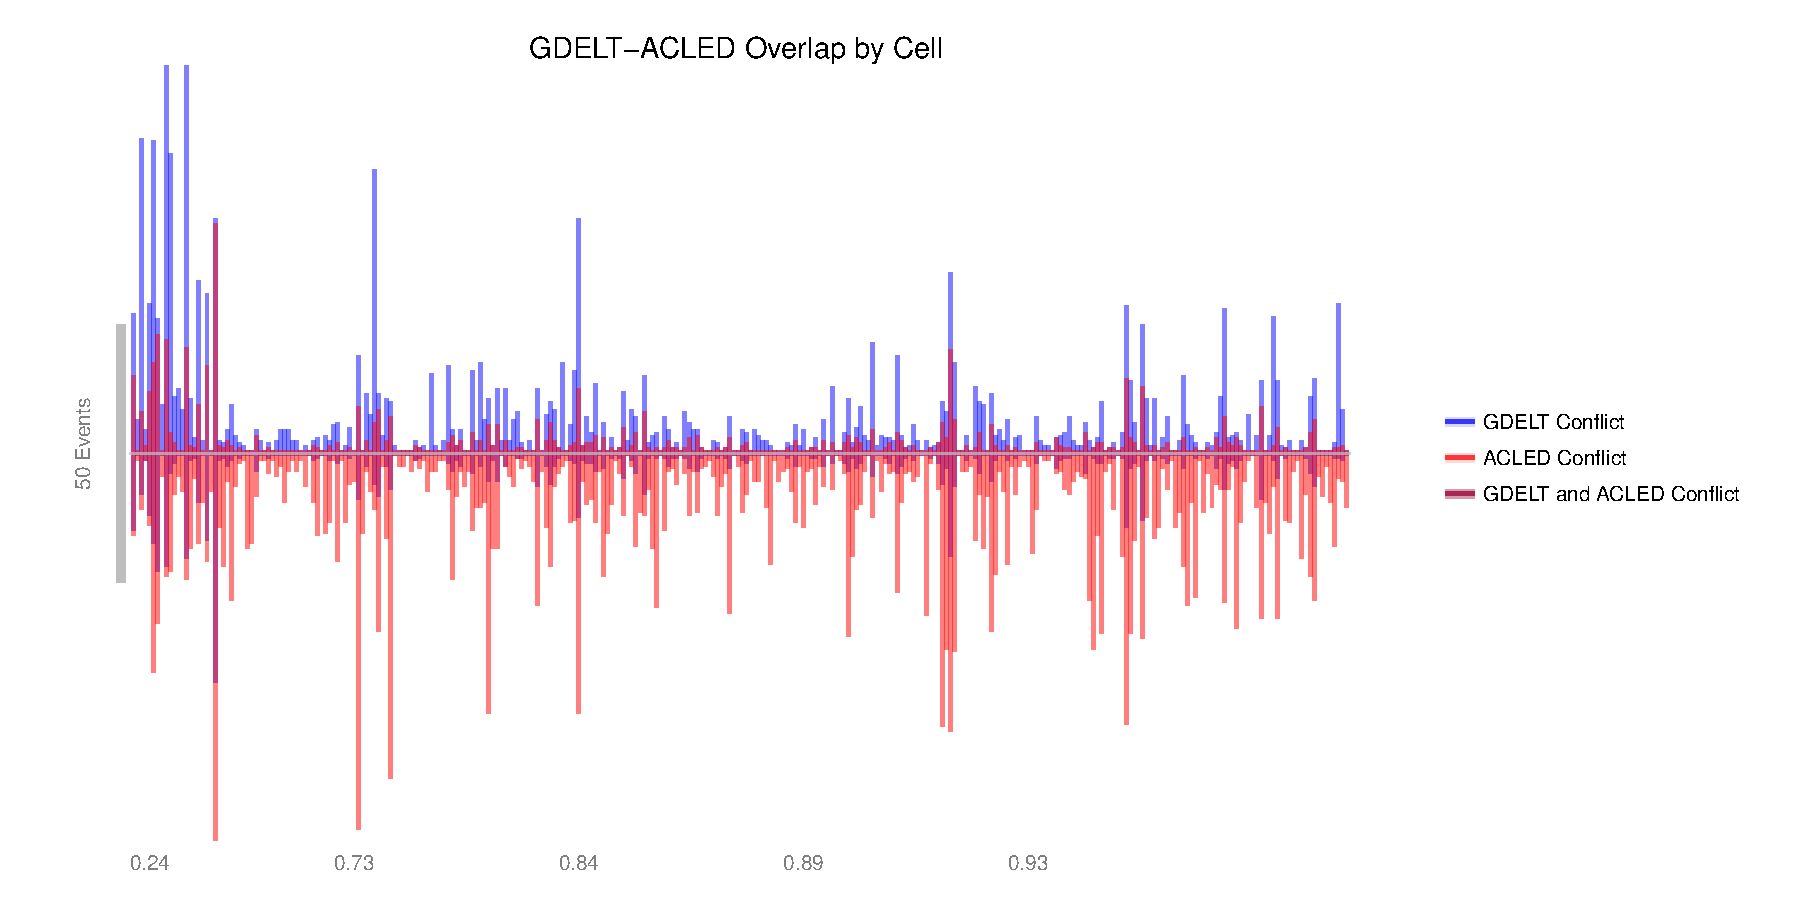
\includegraphics[width = 1 \textwidth]{spaceACLED.pdf}\\
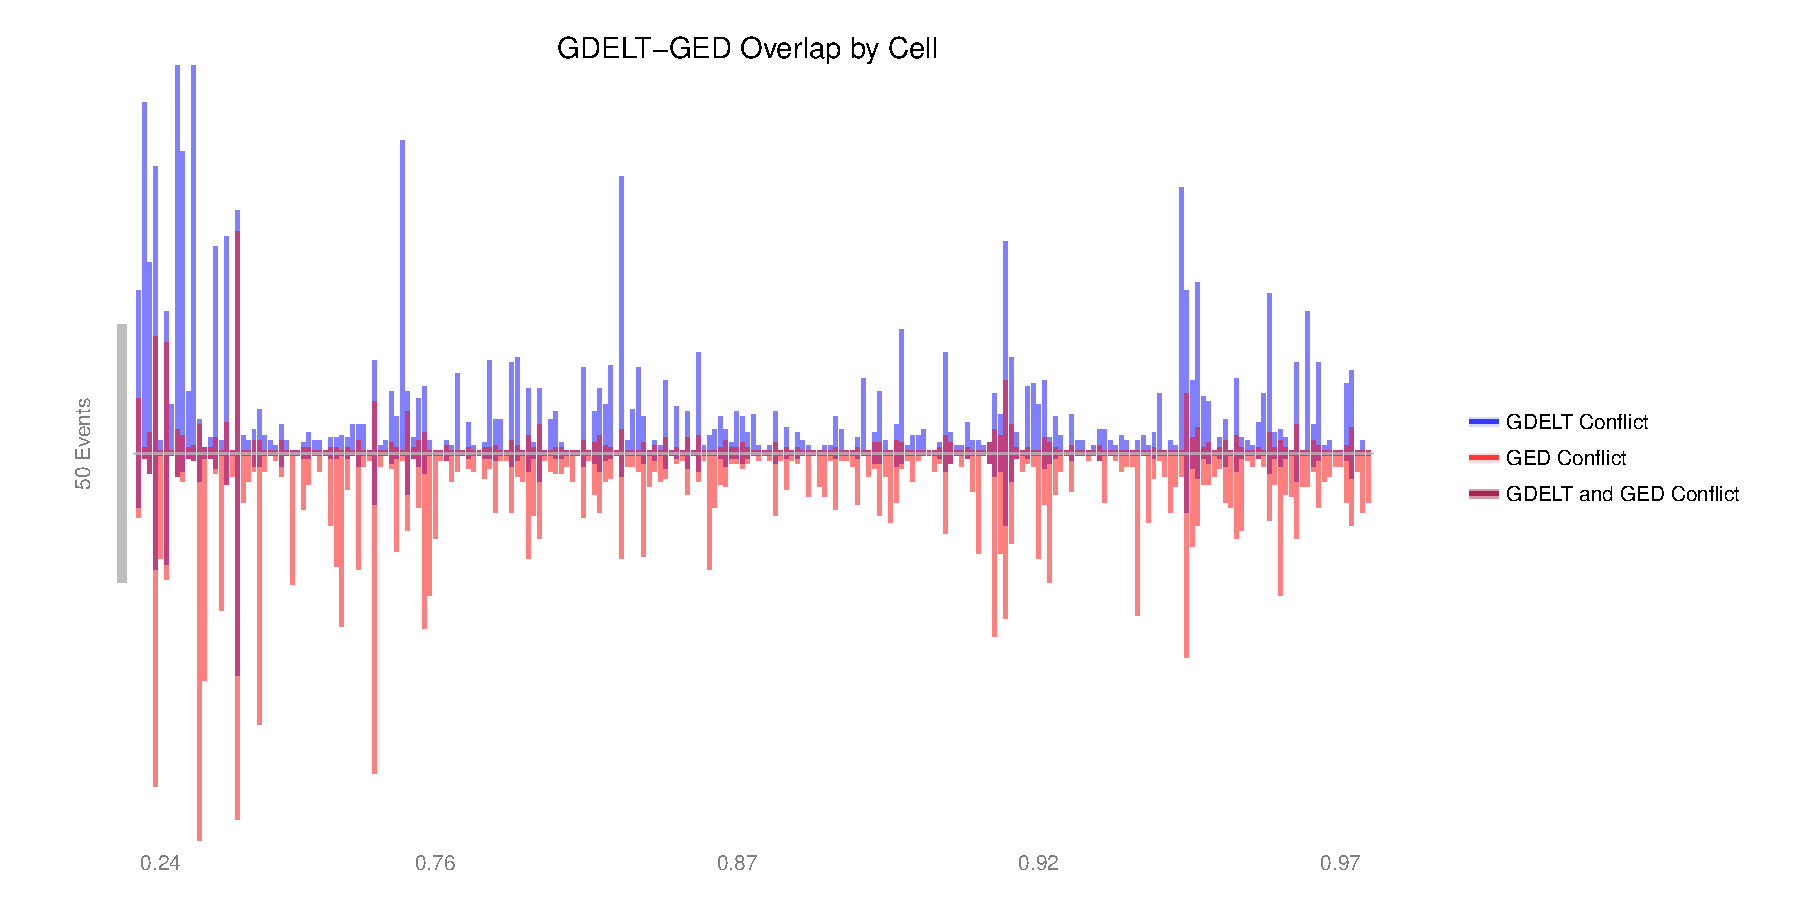
\includegraphics[width = 1 \textwidth]{spaceGED.pdf}
\caption{Grid-cell events over logged and normalized capital distance.}\label{fig:correlations_space}
\end{figure}

The non-overlapping parts of the bars show that there are a large number of cases that are coded as conflict by ACLED or GED, but which are not captured by GDELT (and, as Appendix D shows, these cases are not due to the wider range of sources used by the hand-coded datasets). No clear trend can be identified when it comes to variation over time (Figure \ref{fig:correlations_time}). Visualizing conflict reports over space shows higher reporting by all datasets in grid-cells close to the capital city, but there is no visually discernible trend in how distance to the capital affects the likelihood of both datasets reporting an event in the same cell-month. We further explore spatial variation in disagreement between the datasets using regression analysis. We create a variable measuring incidences where a cell-month was coded as conflict by one of the human-coded datasets, but not GDELT, or by GDELT but not by the human-coded dataset. We regress this variable on the distance from the capital (logged and normalized to the 0-1 interval by country), controlling for logged population and the amount of rugged terrain within a given cell. The results are shown in Table \ref{tab:regression1}.


% Table created by stargazer v.4.5.2 by Marek Hlavac, Harvard University. E-mail: hlavac at fas.harvard.edu
% Date and time: Sat, Dec 21, 2013 - 11:43:23
\begin{table}[!htbp] \centering 
\begin{tabular}{@{\extracolsep{5pt}}lcccc} 
\\[-1.8ex]\hline 
\hline \\[-1.8ex] 
 & \multicolumn{2}{c}{\textit{GDELT-ACLED}} & \multicolumn{2}{c}{\textit{GDELT-GED}}\\ 
\cline{2-5} 
\\[-1.8ex] & GDELT = 1, & GDELT = 0, & GDELT = 1, & GDELT = 0 \\ 
\\[-2.8ex] & ACLED = 0 & ACLED = 1 & GED = 0 & GED = 1 \\ 
\\[-1.8ex] & (1) & (2) & (3) & (4)\\ 
\hline \\[-1.8ex] 
 Distance to Capital & $-$3.74$^{***}$ & 1.08$^{***}$ & $-$3.86$^{***}$ & 1.52$^{***}$ \\ 
  & (0.20) & (0.16) & (0.18) & (0.20) \\ 
  & & & & \\ 
 Population & 0.68$^{***}$ & 0.66$^{***}$ & 0.73$^{***}$ & 0.71$^{***}$ \\ 
  & (0.02) & (0.01) & (0.02) & (0.02) \\ 
  & & & & \\ 
 \% Mountainous & 0.69$^{***}$ & 0.66$^{***}$ & 0.63$^{***}$ & 0.57$^{***}$ \\ 
  & (0.09) & (0.06) & (0.09) & (0.07) \\ 
  & & & & \\ 
 Constant & $-$8.32$^{***}$ & $-$11.22$^{***}$ & $-$9.82$^{***}$ & $-$13.25$^{***}$ \\ 
  & (0.53) & (0.36) & (0.68) & (0.52) \\ 
  & & & & \\ 
\hline \\[-1.8ex] 
Observations & 547,812 & 547,812 & 547,812 & 547,812 \\ 
\hline 
\hline \\[-1.8ex] 
\textit{Note:}  & \multicolumn{4}{r}{$^{*}$p$<$0.1; $^{**}$p$<$0.05; $^{***}$p$<$0.01} \\ 
			& \multicolumn{4}{r}{Country-level fixed effects not shown.} \\ 
\normalsize 
\end{tabular} 
  \caption{Logistic regression results: event record disagreement by cell-month.}\label{tab:regression1}
\end{table} 

Controlling for population, we find clear evidence for geographic bias in GDELT. Distance from the capital decreases GDELT coverage as compared to the human coded datasets (Models 2 and 4), whereas the opposite is true if we move closer to the capital (Models 1 and 3). If we assume that human geo-referencing is more accurate (which we believe is a reasonable assumption), these results are consistent with GDELT not being able to geo-reference event accurately, and wrongly placing them near the capital. 

Even if capital bias exists in GDELT, is there reason to worry? In other words, do these misallocated events in GDELT fundamentally change the results we obtain based on these data? To analyze this, we estimated simple structural models using the different datasets in our study. Again, we stick to a binary dependent variable (violence in cell-month). Following standard methodology, we include both the spatial and the temporal lag of violence, both measured in the month before, as well as control variables for population and mountainous terrain. Of particular interest here is the coefficient linking geographic remoteness, as measured by distance to the capital, to the presence of conflict in a given grid-month. Table \ref{tab:regression2} shows the results. 

Most coefficients behave as expected and are consistent across the datasets. For example, violence is more likely to happen in cells with high population or mountainous terrain, and in those which experienced conflict in the month before. However, different datasets seem to give different answers when it comes to the effect of remoteness on violence. The human-coded datasets (ACLED and GED, Models 5 and 6) confirm the frequent finding that violence is more likely in remote areas of a country. This finding has been established with a number of data collections other than ACLED and GED \citep{buhaug06localdeterminants, buhaug08disaggregating}. Results based on GDELT, however, suggest exactly the opposite (Model 7), and show that violence according to GDELT is more likely to occur close to the capital. We take this as clear evidence for a capital-centric geocoding pattern in GDELT, and this geographic bias, as compared to existing datasets on violence, is something that must be taken into account. As we have shown above, an analysis of the location of violence based on GDELT can lead to findings going squarely against many existing works, and this gives significant reason for caution when considering GDELT for micro-level studies of civil war.


% Table created by stargazer v.4.5.2 by Marek Hlavac, Harvard University. E-mail: hlavac at fas.harvard.edu
% Date and time: Sat, Feb 08, 2014 - 11:02:19
\begin{table}[!htbp] \centering 
\begin{tabular}{@{\extracolsep{5pt}}lccc} 
\\[-1.8ex]\hline 
\hline \\[-1.8ex] 
 & \multicolumn{3}{c}{\textit{Dependent variable:}} \\ 
\cline{2-4} 
\\[-1.8ex] & ACLED Conflict & GED Conflict & GDELT Conflict \\ 
\\[-1.8ex] & (5) & (6) & (7)\\ 
\hline \\[-1.8ex] 
 Conflict$_{(t-1)}$ & 2.60$^{***}$ & 2.63$^{***}$ & 2.86$^{***}$ \\ 
  & (0.04) & (0.05)  & (0.05) \\ 
  & & & \\ 
 Spatial lag$_{(t-1)}$ & 0.06$^{***}$ & 0.13$^{***}$ & $-$0.004 \\ 
  & (0.003) & (0.01) & (0.004) \\ 
  & & & \\ 
 Distance to capital & 0.14 & 1.18$^{***}$ & $-$2.41$^{***}$ \\ 
  & (0.15) & (0.18) & (0.18) \\ 
  & & & \\ 
 Population & 0.60$^{***}$ & 0.65$^{***}$ & 0.68$^{***}$ \\ 
  & (0.01) & (0.02) & (0.02) \\ 
  & & & \\ 
 \% Mountainous & 0.44$^{***}$ & 0.31$^{***}$ & 0.48$^{***}$ \\ 
  & (0.06) & (0.07) & (0.08) \\ 
  & & & \\ 
 Constant & $-$10.24$^{***}$ & $-$12.05$^{***}$ & $-$9.80$^{***}$ \\ 
  & (0.36) & (0.44) & (0.51) \\ 
  & & & \\ 
\hline \\[-1.8ex] 
Observations & 547,812 & 547,812 & 547,812 \\ 
Log Likelihood & $-$26,121.86 & $-$19,047.40 & $-$14,483.13 \\ 
Akaike Inf. Crit. & 52,303.71 & 38,154.80 & 29,026.27 \\ 
\hline 
\hline \\[-1.8ex] 
\textit{Note:}  & \multicolumn{3}{r}{$^{*}$p$<$0.1; $^{**}$p$<$0.05; $^{***}$p$<$0.01} \\ 
			& \multicolumn{3}{r}{Country-level fixed effects not shown.} \\ 
\normalsize 
\end{tabular} 
  \caption{Logistic regression results. Dependent variable: Occurrence of violence in cell/month.} \label{tab:regression2} 

\end{table} 

\section*{Conclusions}

Machine coding of event datasets can process large amounts of reports in little time, and thus have some advantages over their human-coded counterparts. In this short article, we have scrutinized the use of one of these event datasets---GDELT---for geo-spatial analysis at the subnational level. Previously, machine-coded event data have been used mostly for the study of international relations, and have been shown to be valid and reliable for this purpose. However, so far there have been few attempts to find out whether relying on machine coding produces data that is equally suitable for analyses at the subnational level. Our analysis reveals a considerable lack of agreement between human-coded and machine coded data. We show that this is largely due to problems in geo-localization. While GDELT seems to track temporal ups and downs in violence as identified by the human-coded datasets, it places a disproportionately high number of events closer to a country's capital, undercounting events in more remote areas. For geospatial analyses of violence, this may be reason to worry. If we cannot be sure that the spatial accuracy of events is within reasonable limits \citep{weidmann15accuracy}, this can make machine-coded event datasets difficult to use for fine-grained analyses of the dynamics of violence on the ground. 

We believe, however, that further work will be able to address these difficulties. As a first step towards more transparency in the machine coding process, datasets should include pointers to the original articles used to code an event. This will enable more thorough validation studies of automatic geo-coding, but also going beyond this. Despite the fact that GDELT is positively correlated with trends identified in other datasets, the overlap is still far from perfect. With traceback information in the dataset, users can go back to the original articles and find out whether, for example, ``protest as coded by GDELT corresponds to the type of ``protest'' they are interested in. Overall, our current recommendation is that GDELT should be viewed at best as a complement, rather than a substitute, for existing event data. GDELT's high level of noise in the data, coupled with geographic accuracy issues suggests that using GDELT instead of a more detailed hand-coded dataset would likely be counterproductive. However, with more work on the refinement of automatic coding, this may well be where event data collection is (and should be) going.

\printbibliography
%\bibliography{paper.bib}
%\bibliographystyle{harvard}

\end{document}
